\documentclass[12pt,a4paper,oneside]{article}
\usepackage[utf8]{inputenc}
\usepackage[czech]{babel}
\usepackage[T1]{fontenc}
\usepackage{float}
\usepackage{graphicx}
\usepackage{index}
\usepackage{listings}
\usepackage{url}
\author{Roman Ondráček}
\title{Dálkové ovládání domácích spotřebičů mobilním telefonem}
% Vytvoření seznamu použitých zkratek
\newindex{zkr}{zdx}{znd}{Seznam použitých zkratek}
\lstset{
    inputencoding=utf8
}
\begin{document}
% Řádkování 1,5
\renewcommand{\baselinestretch}{1.5}
% Vynechání číslování
\pagestyle{empty}
% Zvětšení oblasti tisku pro tuto stránku
\enlargethispage{60mm}
\begin{center}
\large \textbf{STŘEDOŠKOLSKÁ ODBORNÁ ČINNOST} \\

\vspace{32mm}
% Český název
\huge \textbf{Dálkové ovládání domácích spotřebičů mobilním telefonem} \\

\vspace{64mm}
\end{center}

\begin{tabbing}
% Nastavení zarážek
\hspace{4mm} \= \hspace{24mm}  \=   \kill
\> \large \textbf{Autor:}  \> \large{Roman Ondráček}                                    \\[4mm]
\> \large \textbf{Škola:}  \> \large{Gymnázium Boskovice, příspěvková organizace}       \\[4mm]
\> \large \textbf{Kraj:}   \> \large{Jihomoravský}                                      \\[4mm]
\> \large \textbf{Obor:}   \> \large{10. Elektrotechnika, elektronika a telekomunikace} \\[24mm]
\> \large \textbf{Boskovice 2017}
\end{tabbing}

\newpage
% Vynechání číslování
\pagestyle{empty}
% Zvětšení oblasti tisku pro tuto stránku
\enlargethispage{60mm}
\begin{center}
\large \textbf{STŘEDOŠKOLSKÁ ODBORNÁ ČINNOST} \\

\vspace{32mm}
% Český název
\huge \textbf{Dálkové ovládání domácích spotřebičů mobilním telefonem} \\
\vspace{16mm}
% Anglický název
\huge \textbf{The remote control of home appliances via a mobile phone} \\

\vspace{24mm}
\end{center}

\begin{tabbing}
% Nastavení zarážek
\hspace{4mm} \= \hspace{24mm}  \=   \kill
\> \large \textbf{Autor:}     \> \large{Roman Ondráček}                                    \\[4mm]
\> \large \textbf{Škola:}     \> \large{Gymnázium Boskovice, příspěvková organizace}       \\[4mm]
\> \large \textbf{Kraj:}      \> \large{Jihomoravský}                                      \\[4mm]
\> \large \textbf{Školitel:}  \> \large{prof. Ing. Václav Říčný, CSc.}                     \\[4mm]
\> \large \textbf{Obor:}      \> \large{10. Elektrotechnika, elektronika a telekomunikace} \\[16mm]
\> \large \textbf{Boskovice 2017}
\end{tabbing}

\normalsize

\newpage

~ \vspace{88mm}

\section*{Prohlášení}

Prohlašuji, že svou práci na téma Dálkové ovládání domácích spotřebičů mobilním telefonem jsem vypracoval samostatně pod vedením prof. Ing. Václava Říčného, CSc. a s použitím odborné literatury a dalších informačních zdrojů, které jsou všechny citovány v práci a uvedeny v seznamu literatury na konci práce. \\
Dále prohlašuji, že tištěná i elektronická verze práce SOČ jsou shodné a nemám závažný důvod proti zpřístupňování této práce v souladu se zákonem č.~121/2000 Sb., o právu autorském, o právech souvisejících s právem autorským a změně některých zákonů (autorský zákon) v platném změní. \\[8mm]
V Boskovicích dne \today \hspace{24mm} Podpis: 

\newpage

~ \vspace{80mm}

\section*{Poděkování}

Děkuji svému školiteli prof. Ing. Václavu Říčnému CSc. za obětavou pomoc a podnětné připomínky, které mi během práce poskytoval. \\
Tato práce byla provedena za finanční podpory Jihomoravského kraje.

\vspace{8mm}
% Loga
\begin{figure}[!htb]
\minipage{0.50\textwidth}
	
\includegraphics[width = 64mm]{img/logo-jmk.pdf} \\[8mm]
	
\includegraphics[width = 64mm]{img/logo-jcmm.jpg}
\endminipage
\minipage{0.50\textwidth}
	
\includegraphics[width = 64mm]{img/logo-vut.pdf}
\endminipage
\end{figure}

\newpage

\section*{Anotace}

Cílem této práce je navrhnout a sestavit chytrou zásuvku, která se ovládá pomocí pomocí SMS a která může spínat odporovou zátěž až 10~A. Součástí mé práce je technická dokumentace výrobku, popis postupu  výroby a samotný výrobek.

\subsection*{Klíčová slova}

GSM; SMS; IQRF; relé

\section*{Annotation}

The goal of this work is to design and build an smart power socket, which is controlled  by a  text message and it can switch resistive loads up to a current 10~A. My work includes a technical documentation, description of a manufacturing process and the product itself.

\subsection*{Keywords}

GSM; text message; IQRF; relay

\newpage

\tableofcontents

\newpage

\section*{Úvod}

\addcontentsline{toc}{section}{Úvod}

V posledních létech je ve středu pozornosti tzv. Internet věcí (IoT) a chytrá domácnost. Na trhu jsou nabízeny chytré zásuvky, které však obvykle ovládány na kratší vzdálenosti a nenabízejí možnost pohodlně a bezpečně je ovládat vzdáleně pomocí mobilního telefonu. \\

Obvykle jsou tyto chytré zásuvky ovládány pomocí komunikace WiFi, která používá kmitočtové pásmo 2,4 GHz. Tato frekvence je hlavně ve městech hodně zarušená, protože  se  používá i pro přenosy jiných dat\cite{wiki-ism-band}. A proto většinou tyto chytré zásuvky lze ovládat pouze v místní síti (LAN). Tento projekt má tedy umožnit ovládat tyto zásuvky (a tedy i elektrické spotřebiče v nich zapojené) z libovolné vzdálenosti. Navržený systém dálkového ovládání pomocí mobilního telefonu by měl, kromě vlastního ovládání, zabezpečit i přenos informace uživateli o aktuálním stavu zásuvky. Cílem projektu je tedy návrh takové dálkově ovládané chytré zásuvky, její realizace a ověření funkčního vzorku. \\

Většina chytrých zásuvek obsahuje pouze jedno relé\cite{teardown-wemo-switch}, protože musí se povinně spínat fáze (spínání nulového vodiče je nepovinné). To přináší problém, protože například ve Francii, kde se stejně jako v České republice použita zásuvka typu E\cite{zasuvka-typ-e}, je zdířka fáze umístěna vpravo nikoliv vlevo jako v České republice\cite{faze-vlevo-nebo-vpravo}. Proto navržené řešení obsahuje i druhé relé  pro spínání nulového vodiče. \\

Pro řešení zadání projektu jsem se rozhodl použít technologii IQRF. Je to technologie vyvinutá českou firmou Microrisc s.r.o., která se poměrně často používá ve světě internetu věcí a jiných systémů pro bezdrátový přenos malých objemů dat. Firma dává k dispozici relativně malé moduly, které je  možno integrovat do konkrétních zákaznických řešení.

\newpage

\section{Návrh hardware}

\subsection{Chytrá zásuvka}

Chytrá zásuvka je napájena ze sítě pomocí modulového spínaného zdroje do desky plošných spojů MEAN WELL IRM-02-5, který má výstupní napětí 5~V a maximální výstupní proud je 400~mA. \\

Chytrá zásuvka je řízena bezdrátovým modulem IQRF DCTR-72DAT, který spíná SMD unipolární tranzistory N-MOSFET BSS138. Ty spínají které spínají cívky dvou relé (jedno je použito pro spínání fáze a druhé relé je použito pro spínání nulového vodiče) OMRON G5Q-1A4-EU. \\

Při rozepnutí proudu v~cívce relé vzniká vlivem její indukčnosti napěťová špička, která může  zničit spínací tranzistor. Proražení tranzistoru lze zabránit diodou paralelně zapojenou k relé, která při rozepnutí relé uzavře obvod kolem indukčnosti. Použil jsem usměrňovací diodu 1N4007. Abych zabránil jiskření na kontaktech relé, jsem použil varistor MOV SR PASSIVES VAR10-250.

\subsubsection{Bezdrátový modul IQRF DCTR-72DAT}

V chytré zásuvce jsem použil bezdrátový modul IQRF DCTR-72DAT, který rovněž vyrábí česká firma MICRORISC s.r.o., která sídlí v Jičíně. Plošný spoj modulu má podobné rozměry jako SIM karta, proto je pro jeho připojení s deskou plošných spojů použit konektor pro SIM karty. \\ 

Modul může vysílat na bezlicenčních pásmech 916~MHz, která je určené pro Ameriku, a 868~MHz, určené pro zbytek světa. Vysílací výkon modulu je 12,5~mW, používá GMSK modulaci. Modul má integrovanou anténu na svém plošném spoji. \\

Pro komunikaci používá tzv. mesh neboli smíšenou topologii. Ta má výhody v~robustnosti a v absenci centrálního prvku. Její nevýhodou je naopak  potřebná ochrana proti zacyklení a  nutnost směrování provozu.  \\

Modul lze napájet napětím 3,1~V až 5,5~V, protože obsahuje LDO napěťový stabilizátor Microchip  MCP1700T-3002E/TT. Dále modul obsahuje mikrokontrolér Microchip PIC16LF1938. Ten užívá operační systém IQRF OS, který za uživatele zajišťuje komunikaci s integrovaným obvodem STMicroelectronics Spirit1. Tento obvod řídí bezdrátový datový přenos a má hardwarovou podporu blokové šifry AES-128. Operační systém dále ovládá integrované periferie (například digitální teploměr). IQRF DPA a uživatelská aplikace. Dále modul obsahuje digitální teploměr Microchip MCP9808E/MC. \\ 

Přestože je v integrovaném obvodu řídící radiovou komunikaci hardwarová podpora šifry AES-128, tak podpora této šifry není v IQRF OS ještě implementována a místo ní se používá upravená bloková šifra XTEA, která je však méně bezpečná.

\subsubsection{Blokové schéma}

\begin{figure}[H]
\centering
\label{fig:blokove-schema-zasuvky}
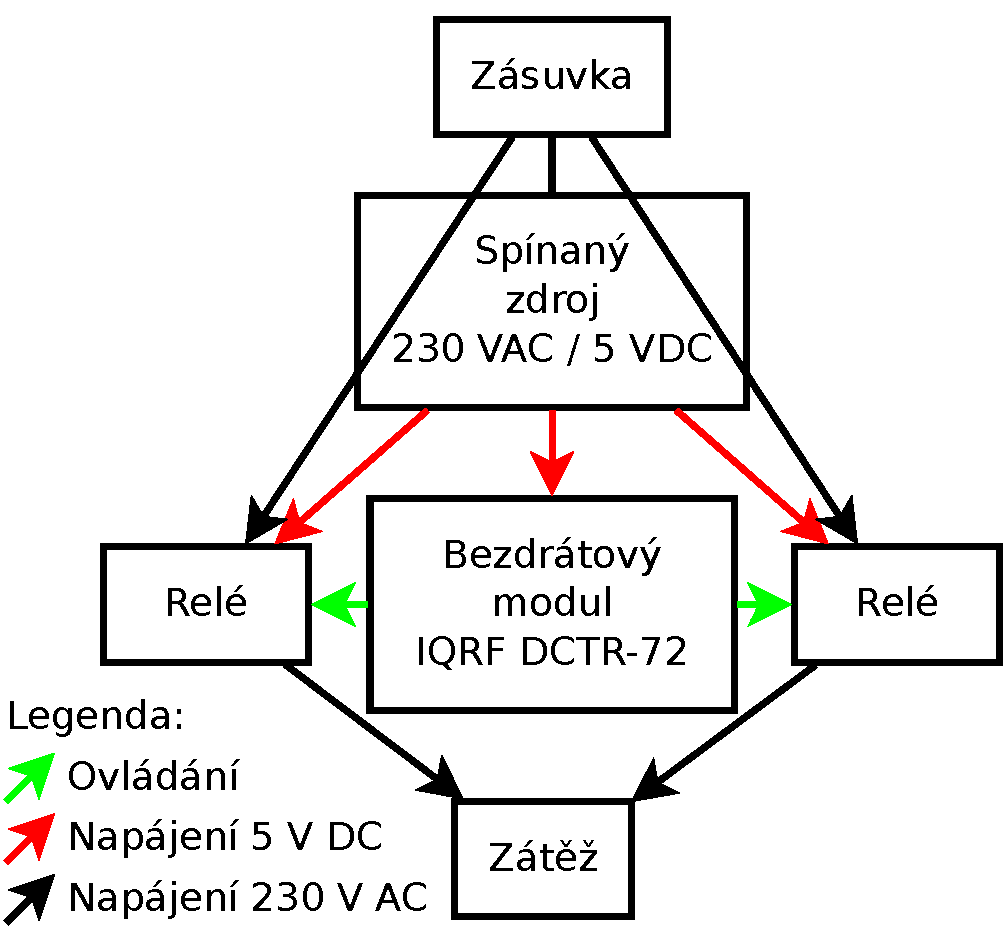
\includegraphics[width = 128mm]{img/blokove-schema-zasuvky.pdf}
\caption{Blokové schéma chytré zásuvky}
\end{figure}

\subsubsection{Obvodové schéma}

\begin{figure}[H]
\centering
\label{fig:schematic}
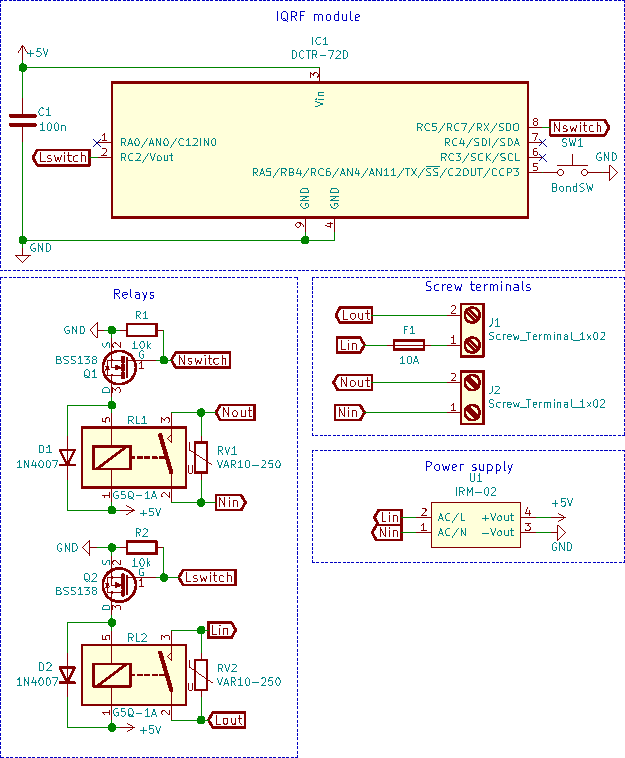
\includegraphics[width = 128mm]{img/schematic.pdf}
\caption{Obvodové schéma chytré zásuvky}
\end{figure}

\subsubsection{Výkres plošného spoje a rozložení součástek}

\begin{figure}[H]
\centering
\label{fig:board}
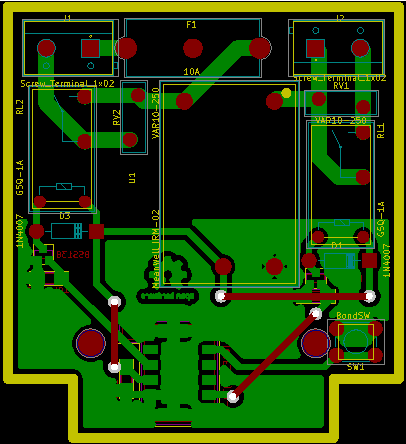
\includegraphics{img/board.pdf}
\caption{Výkres plošného spoje chytré zásuvky}
\end{figure}

\begin{figure}[H]
\centering
\label{fig:components}
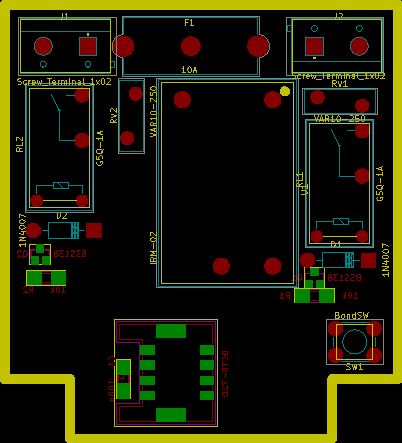
\includegraphics{img/components.pdf}
\caption{Rozložení součástek na desce plošného spoje chytré zásuvky}
\end{figure}

\subsubsection{Rozpiska součástek}

\begin{table}[H]
	\centering
	\begin{tabular}{|l|l|}
		\hline 
		\textbf{Značka} & \textbf{Jméno součástky} \\ 
		\hline 
		\hline 
		~ & Krabička COMBIPLAST CP-Z-27/B \\ 
		\hline 
		C1 & Keramický SMD\index[zkr]{SMD!Surface-mounted device|textit} 1206 kondenzátor 100~nF \\ 
		\hline 
		D1, D2 & Dioda 1N4007 \\ 
		\hline 
		F1 & Tavná keramická pojistka 10~A 250~VAC \\ 
		\hline 
		IC1 & Bezdrátový modul IQRF DCTR-72DAT \\ 
		\hline 
		~ & Konektoru IQRF KON-SIM-01 pro IC1 \\ 
		\hline 
		J1, J2 & Svorkovnice do DPS DEGSON DG300-7.5-02P \\ 
		\hline 
		Q1, Q2 & N-MOSFET BSS138 \\ 
		\hline 
		R1, R2 & Rezistor SMD 1206 10~k$\Omega$ \\ 
		\hline 
		RL1, RL2 & Relé OMRON G5Q-1A4-EU 5VDC \\ 
		\hline 
		RV1, RV2 & MOV varistor SR PASSIVES VAR10-250 \\ 
		\hline 
		SW1 & Mikrospínač THT 6$\times$6~mm \\ 
		\hline 
		U1 & Spínaný zdroj MEAN WELL IRM-02-5 \\ 
		\hline 
	\end{tabular}
	\caption{Rozpiska součástek chytré zásuvky}\label{table:rozpiska-soucastek}
\end{table}

\subsection{Brána}

Pro bránu jsem použil linuxový jednodeskový počítač Raspberry Pi 2 model B. Bezdrátový modul IQRF DCTR-72DAT je k bráně připojen přes sběrnici SPI pomocí adaptéru IQRF KON-RASP-01. Pro komunikaci s GSM sítí lze použít USB GSM/3G modem (například Huawei E3131) nebo starší mobilní telefon (například Samsung Star II nebo Samsung Galaxy Gio). Brána se napájí pomocí externího spínaného zdroje s microUSB konektorem, který má výstupní napětí 5~V a maximální výstupní proud 2~A.

\section{Návrh software}

\subsection{Chytrá zásuvka}

Software chytré zásuvky je psán v programovacím jazyce C. Pro práci s periferiemi bezdrátového modulu je použita sada funkcí IQRF OS. 

\subsubsection{IQRF OS}

IQRF OS je sada funkcí psaná v programovacím jazyce C, které může uživatel ze svého programu volat pomocí hlavičkových souborů IQRF-functions.h, IQRF-macros.h, IQRF-memory.h a template-basic.h. Tyto funkce řídí komunikaci s integrovaným obvodem, který se stará o rádiovou komunikaci, o komunikaci v mesh síti, o komunikaci přes sběrnici SPI, o práci s pamětmi RAM, EEPROM, o čtení hodnot z integrovaného teplotního senzoru, o čtení hodnot z analogově digitálního převodníku, o generování PWM výstupu, o inicializaci vstupních a výstupních vývodů mikrokontroléru, o čtení hodnot z vstupních vývodů mikrokontroléru, o spínání výstupních pinů mikrokontroléru a o správu LED diod, které jsou integrovány v bezdrátovém modulu. 

\subsubsection{IQRF DPA}

IQRF DPA je vrstva nad IQRF OS, která se stará o protokol komunikace IQRF bezdrátových modulů. IQRF DPA má pevně danou strukturu paketů, kterou naleznete v tabulce. Centrální prvek v IQRF mesh síti se jmenuje koordinátor, který je umístěn v bráně. Koordinátor má se své paměti EEPROM uložené informace o dalších bezdrátových modulech, se kterými má komunikovat. Pokud koordinátor přijme data od bezdrátového modulu, jehož informace nemá uložené v EEPROM paměti, tak data ignoruje.

\subsection{Brána}

V bráně běží linuxová distribuce Raspbian, což je speciálně upravená linuxová distribuce pro jednodeskový počítač Raspberry Pi. Tato linuxová distribuce je odvozená od linuxové distribuce Debian, která je jedna z nejpoužívanějších linuxových distribucích. Software brány je psán v skriptovacím jazyce Python. Abych si byl jistý, že všechny komponenty softwaru brány fungují, tak jsem pomocí nástroje unittest psal unit testy, které testují důležité komponenty (například čtení konfiguračního souboru). \\

Konfigurační soubor softwaru brány je psán v datovém formátu JSON. A níže naleznete ukázkový konfigurační soubor.

\subsubsection{AT příkazy}

AT příkazy jsou sada příkazů, které se používají pro komunikaci s GSM modemem. Dříve se AT příkazům říkalo Hayesovy příkazy. AT příkazy vymyslel Dennis Hayes pro svůj Hayes Smartmodem 300. Pojmenování AT příkazy vzniklo podle slova \textbf{AT}tention, což v češtině znamená pozor, upozornit. \\

Základní AT příkaz je příkaz \textit{AT}, který odpoví OK, pokud je vše v pořádku. Příkaz \textit{ATI} vypisuje informace o modemu (například výrobce a model). Pomocí příkazu \textit{AT+CMGF=1} nastavím textový ASCII přenos dat. \\

Pokud je SIM karta chráněna PIN kódem, tak SIM kartu odemknu pomocí příkazu \textit{AT+CPIN=PIN-SIM-KARTY} a poté pomocí příkazu \textit{AT+CPIN?} ověřím, zda byl zadán správný PIN kód. \\

Pomocí příkazu \textit{AT+CMGL=”ALL”} přečtu každou sekundu všechny SMS zprávy, které jsou uloženy na SIM kartě. Odpověď vypadá takto:

\textit{+CMGL: číslo SMS zprávy,"stav zprávy (přečteno/nepřečteno)","telefonní číslo odesílatele",,"datum a čas přijetí SMS zprávy" \\ Text \\ OK}. 
Pomocí příkazu \textit{AT+CMGS="telefonní číslo příjemce" \\ Text <26>} odešlu SMS zprávu.

Pomocí příkazu \textit{ATD+420123456789;} vytočím telefonní číslo +420123456789. Poté pomocí příkazu \textit{AT+CHUP} zavěsím hovor.

\begin{table}[H]
	\centering
	\begin{tabular}{|l|l|}
		\hline 
		\textbf{Příkaz} & \textbf{Popis} \\ 
		\hline 
		\hline 
		AT & Základní AT příkaz \\ 
		\hline 
		ATI & Vypíše informace o modemu \\ 
		\hline 
		AT+CPIN=1234 & Odemkne SIM kartu pomocí PINu 1234 \\ 
		\hline 
		AT+CPIN? & Odpoví, zda-li je PIN v pořádku \\ 
		\hline 
		AT+CMGF=1 & Nastavíme testový ASCII přenos dat \\ 
		\hline 
		AT+CMGL=”ALL” & Přečte všechny SMS zprávy \\ 
		\hline 
		AT+CMGS="telefonní číslo příjemce"& Odeslání SMS zprávy \\ 
		\hline 
		ATD+420123456789; & Vytočí číslo +420123456789 \\ 
		\hline 
		AT+CHUP & Zavěšení hovoru \\ 
		\hline 
	\end{tabular}
	\caption{Seznam použitých AT příkazů}\label{table:at-prikazy}
\end{table}

\newpage

\section{Použitá vývojová prostředí}

Pro vybraný bezdrátový modul je pouze k dispozici zdarma stažitelné vývojové prostředí IQRF IDE, které je bohužel pouze pro operační systém Microsoft Windows. Uživatelé Apple OS X nebo libovolné linuxové distribuce nemohou vyvíjet software pro tyto bezdrátové moduly.

Software, který běží v bráně jsem psal v vývojovém prostředí Atom IDE, které je open-source a je multiplatformní.

\newpage

\section{Technické parametry}

\subsection{Chytrá zásuvka}

\begin{table}[H]
	\centering
	\begin{tabular}{lr}
		\hline 
		\textbf{Technické parametry} & ~ \\ 
		\hline 
		\hline 
		\textbf{Rozměry} & 7$\times$12$\times$4,5~cm \\ 
		\textbf{Hmotnost} & x~g \\ 
		\hline
		\textbf{Elektrické parametry} \\ 
		\hline 
		\hline 
		\textbf{Napájecí napětí} & 90~V až 250~V AC \\ 
		\textbf{Maximální spotřeba} & 400~mA \\ 
		\textbf{Maximální spínatelný proud} &  10~A \\ 
		\hline 
		\textbf{Ostatní parametry} \\ 
		\hline 
		\hline 
		\textbf{Přenos dat} & bezdrátově na frekvenci 868~MHz \\ 
		\textbf{Protokol} & IQRF DPA \\ 
	\end{tabular}
	\caption{Parametry chytré zásuvky}\label{table:parametry/chytra-zasuvka}
\end{table}

\subsection{Brána}

\newpage

\section*{Závěr}

\addcontentsline{toc}{section}{Závěr}

Výsledkem této práce je funkční chytrá zásuvka, která splňuje veškeré požadavky.

\newpage

\printindex[zkr]

\addcontentsline{toc}{section}{Seznam použitých zkratek}

\newpage

\begin{thebibliography}{99}

\addcontentsline{toc}{section}{Seznam použité literatury}

\bibitem{wiki-ism-band}
Wikipedia. ISM Band \emph{Wikipedia} [online]. [cit. 2016-01-08]. \\ Dostupné z: \url{https://en.wikipedia.org/wiki/ISM\_band}

\bibitem{hayes-command-set}
Wikipedia. Hayes command set \emph{Wikipedia} [online]. [cit. 2016-01-08]. \\ Dostupné z: \url{https://en.wikipedia.org/wiki/Hayes\_command\_set}

\bibitem{iqrf-os}
MICRORISC. Operating system \emph{IQRF} [online]. Jičín, 2016 [cit. 2017-01-09]. \\ Dostupné z: \url{http://iqrf.org/technology/operating-system}

\bibitem{iqrf-dpa}
MICRORISC. DPA \emph{IQRF} [online]. Jičín, 2016 [cit. 2017-01-09]. \\ Dostupné z: \url{http://iqrf.org/technology/dpa}

\bibitem{iqrf-dctr-72d-datasheet}
MICRORISC. Datasheet DCTR-72D \emph{IQRF} [online]. Jičín, 2016 [cit. 2017-01-09]. \\ Dostupné z: \url{http://iqrf.org/weben/downloads.php?id=337}

\bibitem{robodoupe-mosfet-a-rele}
Jiri Bezstarosti. Tranzistor jako spínač \emph{Robodoupě} [online]. 2012 [cit. 2017-01-09]. \\ Dostupné z: \url{http://robodoupe.cz/2012/tranzistor-jako-spinac/}

\bibitem{faze-vlevo-nebo-vpravo}
Jaroslav Borovec. Fáze vlevo nebo vpravo, v čem tkví nebezpečí? \emph{Eletrika.cz} [online]. 2009 [cit. 2017-01-09]. \\ Dostupné z: \url{http://elektrika.cz/clanky/faze-vlevo-nebo-vpravo-v-cem-tkvi-nebezpeci}

\bibitem{zasuvka-typ-e}
Oldřich Mrázek. Přehled zásuvek používaných ve světě - Typ E \emph{HW Server} [online]. 2009 [cit. 2017-01-09]. \\ Dostupné z: \url{http://zasuvky.hw.cz/index2.php#E}

\bibitem{teardown-wemo-switch}
Brian Dipert. Teardown: WeMo Switch is highly integrated \emph{EDN} [online]. 2015 [cit. 2017-01-09]. \\ Dostupné z: \url{http://www.edn.com/design/consumer/4440797/Teardown--WeMo-Switch-is-highly-integrated}
\end{thebibliography}

\newpage

\listoffigures

\addcontentsline{toc}{section}{Seznam obrázků}

\listoftables

\addcontentsline{toc}{section}{Seznam tabulek}

\end{document}